\documentclass{beamer}

\usepackage{listings}
\usepackage{url}
\usepackage{graphicx}
\usepackage{tikz}
\usepackage{caption}
\usepackage{subcaption}

\usetheme{Berlin}
\usecolortheme{beaver}

\title{Kurs i NumPy med NumFys}
\author{Thorvald Ballestad og Jenny Lunde}
\date{2. mars 2021}
\logo{\url{thorvald.tb@gmail.com}
\includegraphics[width=0.75cm]{numfys.png}}

\lstset{
  frame=single,
  language=python,
  breaklines=true,
  numbers=left,
  numberstyle=\tiny,
  commentstyle=\color[gray]{0.4},
}

\begin{document}
\frame{\titlepage}

\frame{\tableofcontents}
%% Intro %% 
\section{Intro og recap}

\begin{frame}[containsverbatim]
	\frametitle{Hvorfor NumPy}
	\begin{itemize}
		\item Gjør det enklere å jobbe med numerikk i Python
			\begin{lstlisting}[language=python]
my_numpy_list*2  // [1,2,4] -> [2,4,8]
my_python_list*2  // [1,2,4] -> [1,2,4,1,2,4]
			\end{lstlisting}
		\item Går \emph{mye} raskere
	\end{itemize}
\end{frame}

\begin{frame}[fragile]
  \frametitle{Litt recap}
  Dette burde (i noen grad) være kjent fra før:\\

  NumPy-array $>$ Python-liste.
  \begin{itemize}
  \item \lstinline{np.linspace(start,end,num_points)}
  \item \lstinline{np.arange(start,stop,step)}
  \end{itemize}

  Operasjoner funker slik de gjør i matte:
  \begin{lstlisting}
    x = np.array([1,2,3])
    my_func(x)  # Returnerer en array der my_func har blitt evaluert for hvert element i x
  \end{lstlisting}
\end{frame}

\begin{frame}[fragile]
  Plotting:
  Vi plotter ved å gi \lstinline{matplotlib} to lister, en med $x$-verdier og en med $y$-verdier.
  \begin{lstlisting}[language=python, breaklines=true, frame=single]
import numpy as np
import matplotlib.pyplot as plt
    
x = np.linspace(-10, 10, 100)  # 100 points from -10 to 10
y = np.sin(x)

plt.plot(x, y, label='sin(x)')
plt.legend()
plt.show()
  \end{lstlisting}
\end{frame}
\begin{frame}
  \centering
  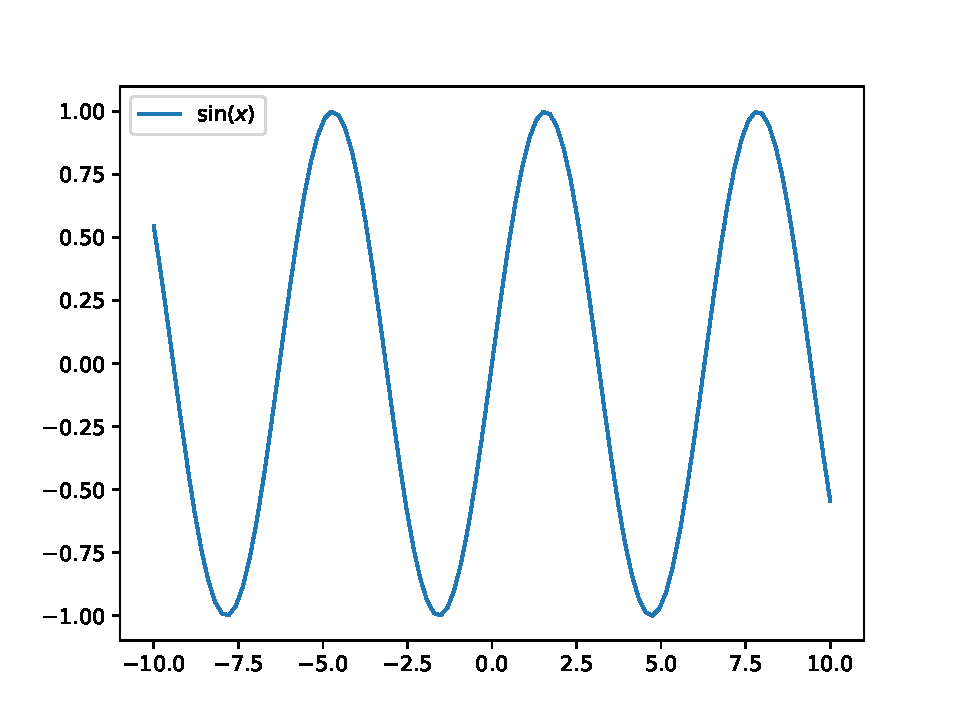
\includegraphics[width=0.75\textwidth]{simple_plot}
\end{frame}
\begin{frame}
  \begin{block}{Oppgave 1 -- The basics}\end{block}
\end{frame}


%% To-dimensjonale arrays %%
\section{To-dimensjonale arrays}

\begin{frame}[fragile]
  \frametitle{To-dimensjonale arrays i NumPy (matriser)}
  NumPy arrays kan ha flere dimensjoner.
  \begin{lstlisting}
data = np.array([[1,2],[3,4]])
# [[1,2],
#  [3,4]]
  \end{lstlisting}
  Funker ellers likt som vanlige arrays.\\
\end{frame}
\begin{frame}[fragile]
  \frametitle{To-dimensjonale arrays i NumPy (matriser)}
  Slicing -- å få ut dataen du vil ha
  \begin{lstlisting}
data = np.array([[1,2,3],
                 [4,5,6]])
data[0]    # First row
data[0,:]  # Also first row
data[:,0]  # First column
###
python_list[start:stop]
  \end{lstlisting}
\end{frame}

\begin{frame}
  \begin{block}{Oppgave 2 -- Matriser}\end{block}
\end{frame}

%% Meshgrid %%
\begin{frame}[fragile]
  \frametitle{Meshgrid}
  \begin{minipage}[b]{.55\textwidth}
  \begin{lstlisting}[title={Meshgrid}]
x = np.linspace(-4, 4, 100);
y = np.linspace(-4, 4, 100);

xx,yy = np.meshgrid(x,y);
  \end{lstlisting}
  \end{minipage}
  \begin{minipage}[b]{.3\textwidth}
  \begin{tikzpicture}
    \draw (0,0) grid (4.9,4.9);
    \draw[->] (0,0) -- (5,0) node[right] {$x$};
    \draw[->] (0,0) -- (0,5) node[above] {$y$};
  \end{tikzpicture}
  \end{minipage}
\end{frame}
\begin{frame}
  \begin{center}
    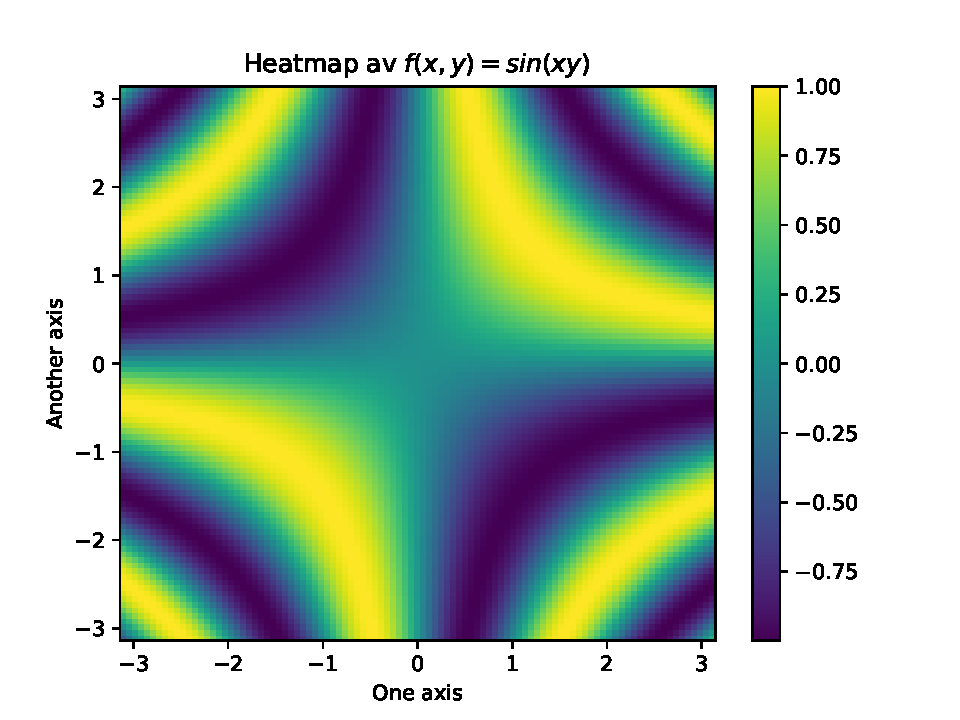
\includegraphics[width=0.75\textwidth]{heatmap}
  \end{center}
\end{frame}
\begin{frame}
  \frametitle{Meshgrid}
  \centering
    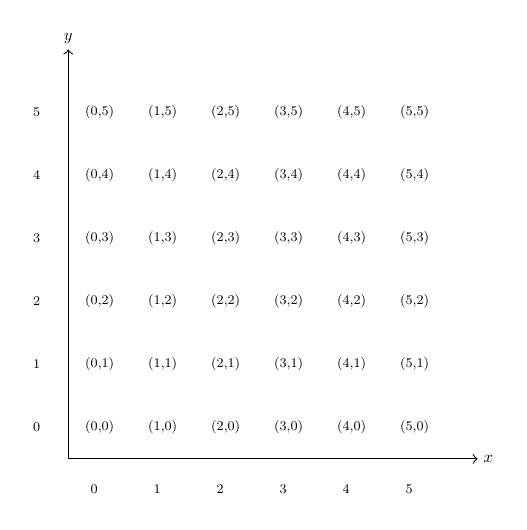
\begin{tikzpicture}[scale=0.8, every node/.style={scale=0.6}]
%    \draw (0,0) grid (4.9,4.9);
    \draw[->] (-0.5,-0.5) -- (6,-0.5) node[right] {$x$};
    \draw[->] (-0.5,-0.5) -- (-0.5,6) node[above] {$y$};


    \foreach \x in {0,...,5}
    \foreach \y in {0,...,5}
    \node at (\x,\y) {\footnotesize(\x,\y)};


    \foreach \x in {0,...,5}
    \node at (\x, -1) {\footnotesize\x\phantom{,0}};

    \foreach \y in {0,...,5}
    \node at (-1, \y) {\footnotesize\y};
  \end{tikzpicture}
\end{frame}

\begin{frame}
  \frametitle{Meshgrid}
  \centering
    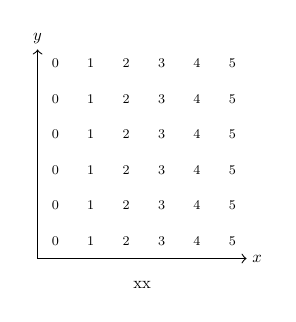
\begin{tikzpicture}[scale=0.45, every node/.style={scale=0.6}]
%    \draw (0,0) grid (4.9,4.9);
    \draw[->] (-0.5,-0.5) -- (5.4,-0.5) node[right] {$x$} node[midway, below, yshift=-10pt]{xx};
    \draw[->] (-0.5,-0.5) -- (-0.5,5.4) node[above] {$y$};



    \foreach \x in {0,...,5}
    \foreach \y in {0,...,5}
    \node at (\x,\y) {\footnotesize\x};
    \end{tikzpicture}
    \qquad
    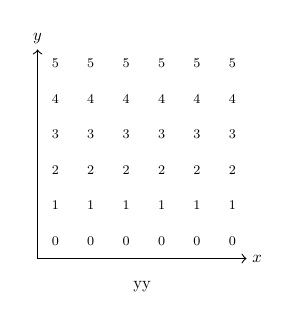
\begin{tikzpicture}[scale=0.45, every node/.style={scale=0.6}]
%    \draw (0,0) grid (4.9,4.9);
    \draw[->] (-0.5,-0.5) -- (5.4,-0.5) node[right] {$x$} node[midway, below, yshift=-10pt]{yy};
    \draw[->] (-0.5,-0.5) -- (-0.5,5.4) node[above] {$y$};


    \foreach \x in {0,...,5}
    \foreach \y in {0,...,5}
    \node at (\x,\y) {\footnotesize\y};
  \end{tikzpicture}
\end{frame}

\begin{frame}
  \begin{block}{Oppgave 3 -- Stepping it up}\end{block}
\end{frame}

%% Plotting i 2D %%
\section{Plotting i 2D}
\begin{frame}
  \frametitle{Plotting i 2D}
  \begin{center}
    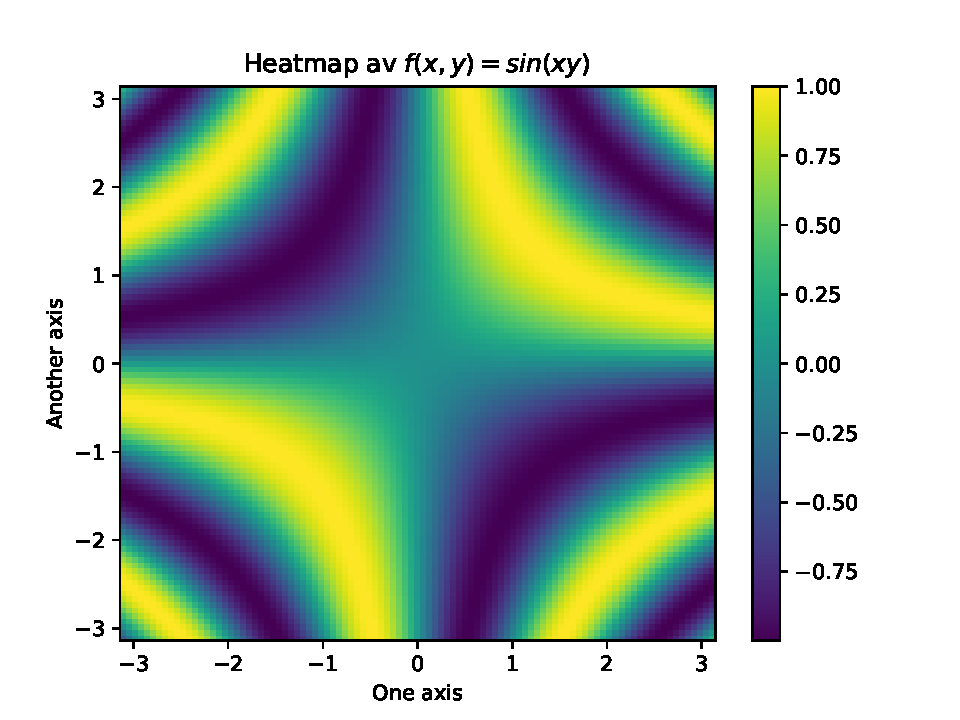
\includegraphics[width=0.75\textwidth]{heatmap}
  \end{center}
\end{frame}

\begin{frame}[fragile]
  \frametitle{Plotting i 2D}
  \begin{minipage}[t]{.45\linewidth}
    \centering
    \textbf{2D}
  \begin{itemize}
  \item pcolormesh
  \item quiver
    {\color{gray}
    \item contour
    \item streamplot
      }
  \end{itemize}
  \end{minipage}
  \begin{minipage}[t]{.45\linewidth}
    \centering
    \textbf{3D}
    \begin{itemize}
      \color{gray}
    \item \lstinline{plot_surface}
    \item \lstinline{contour}
    \item \lstinline{plot} (med x,y,z)
    \item \url{matplotlib.org/mpl_toolkits/mplot3d/tutorial.html} for liste.
    \end{itemize}
  \end{minipage}
\end{frame}

\begin{frame}
  \begin{figure}
    \begin{subfigure}[b]{0.49\textwidth}
      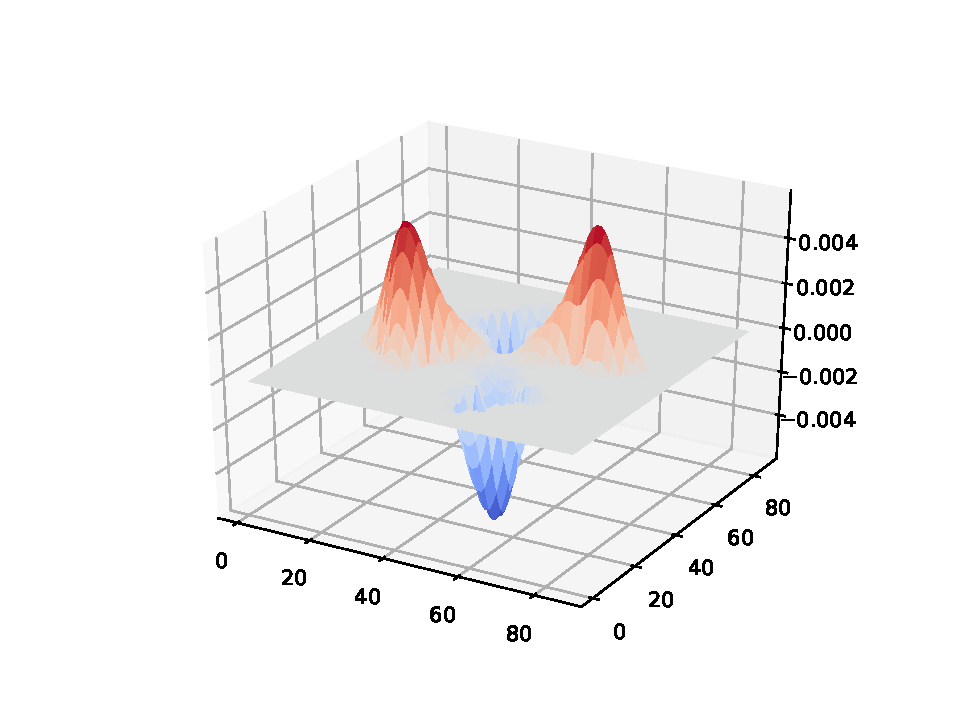
\includegraphics[width=\textwidth]{mode_4.pdf}
    \end{subfigure}
    \begin{subfigure}[b]{0.49\textwidth}
      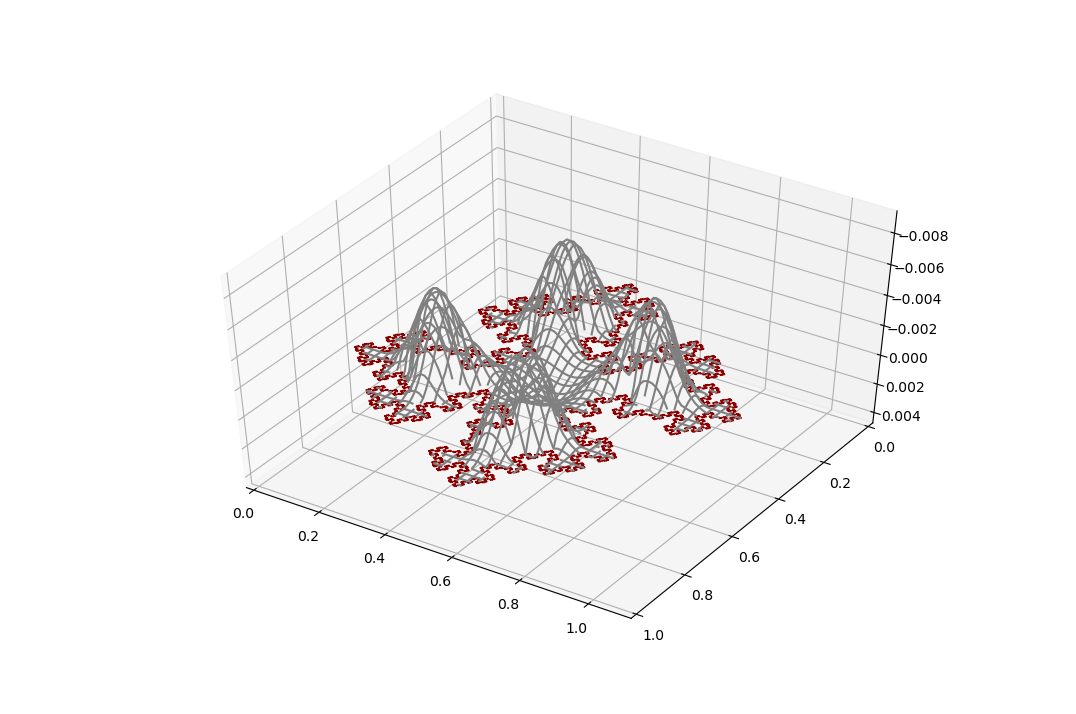
\includegraphics[width=\textwidth]{wireframe_stylish.png}
    \end{subfigure}
  \end{figure}
\end{frame}

\begin{frame}[fragile]
  \frametitle{pcolormesh}
  Heatmap som indikerer verdien til en tovariabel skalar funksjon.
  \begin{lstlisting}
x = np.linspace(-10, 10, 100)
y = np.linspace(-10, 10, 100)
xx,yy = np.meshgrid(x,y)

plt.pcolormesh(xx,yy,xx**2/3 + yy**2)
plt.colorbar()
  \end{lstlisting}
    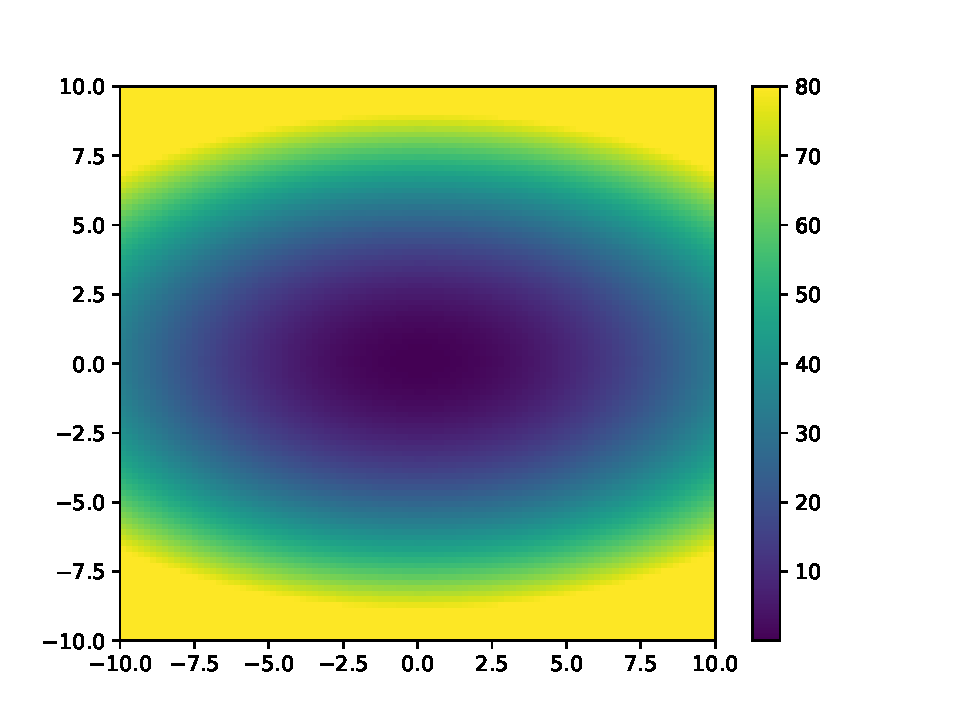
\includegraphics[width=0.3\textwidth]{colormap2}
\end{frame}
\begin{frame}[fragile]
  \frametitle{quiver}
  Indikerer størrelse og retning på en tovariabel vektorfunksjon.
  \begin{lstlisting}
x = np.linspace(-10, 10, 10)
y = np.linspace(-10, 10, 10)
xx,yy = np.meshgrid(x,y)

plt.quiver(xx,yy, xx, yy)
  \end{lstlisting}
      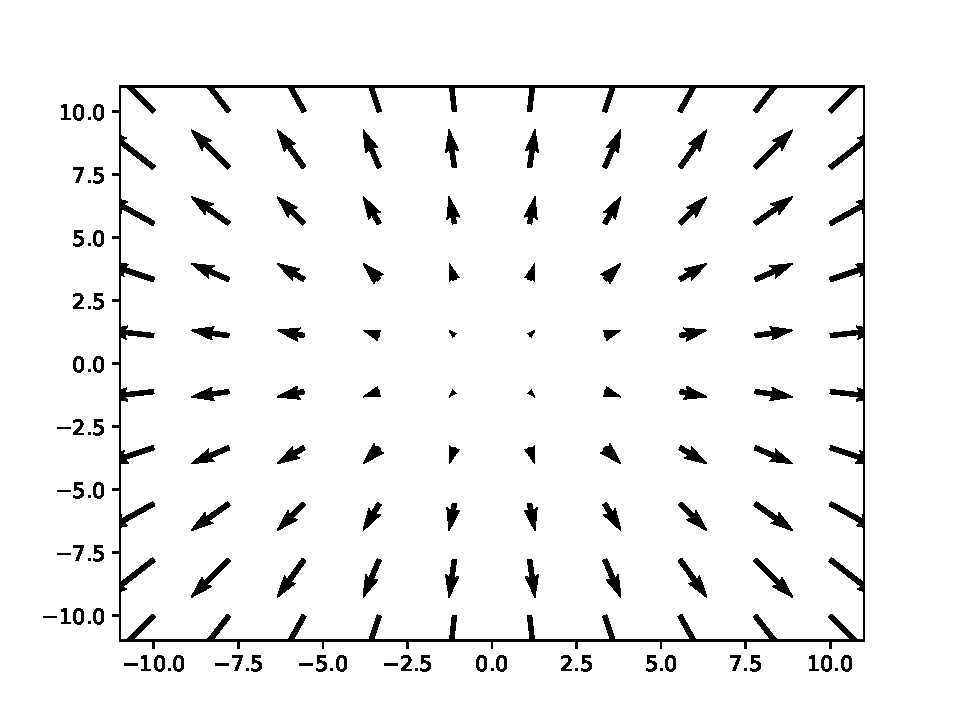
\includegraphics[width=0.3\textwidth]{quiver}
\end{frame}

\begin{frame}
  \begin{block}{Oppgave 4 -- Plotting i 2D}\end{block}
\end{frame}

%% Lese fra fil %%
\section{Lese fra fil}
\begin{frame}[fragile]
  \frametitle{Lese fra fil}

  Å lese data fra fil krever litt jobb for å legge inn dataen på rikitig måte i python-variabler.
  NumPy har en nyttig funksjon, \lstinline{loadtxt}, som gjør dette enkelt.
  \begin{lstlisting}
# Assume my_data.txt has format
# second  temperature  wind_speed

time, temp, wind = np.loadtxt('my_data.txt', unpack=True)
# Notice the unpack=True option
  \end{lstlisting}
\end{frame}


\section{Ressurser}
\begin{frame}
  \frametitle{Nyttige ressurser}
  \begin{itemize}
  \item \url{www.numfys.net}\\
    Inneholder mange notebooks på alle nivåer.
    \begin{itemize}
    \item \url{http://numfys.net/kurs}
    \item \url{http://nbviewer.jupyter.org/urls/www.numfys.net/media/notebooks/intermediate_plotting_final.ipynb}
    \item \url{http://nbviewer.jupyter.org/urls/www.numfys.net/media/notebooks/NumpyIntermediate.ipynb}
    \end{itemize}

  \item \url{http://numpy.org/devdocs} (like greit å søke etter den funksjonen du lurer på, NumPy docs kommer ofte høyt i resultatlista)
  \end{itemize}
\end{frame}
\end{document}
